
A subdivision surface is the limit surface resulting from the
application of a \italic{subdivision scheme} to a control polyhedron
(see Fig.\ref{fig:teaser}). During this process the polygon base
mesh is recursively subdivided and the mesh geometry is progressively
modified according to subdivision rules. A subdivision scheme is
characterized by a refinement operator that acts on the connectivity
by subdividing the mesh, and by a smoothing operator that modifies the
geometry. 

Figure. \ref{fig:RefSchemes} introduces several refinement schemes in
practice. Some general properties of these refinement schemes are
\italic{regular pattern}, \italic{rotationally symmetric} and well
\italic{defined footprint} of each vertex in the
range. Figure. \ref{fig:PQQMap} demonstrates the functional map from
the footprint in the domain mesh to the vertex in the range mesh of
the primal quadrilateral quadrisection scheme. The geometry rules of a
specific refinement scheme is hence defined according to the
corresponding functional maps.

\begin{figure}
  \centering
  \subfigure[Primal quadrilateral quadrisection.] {
    \includegraphics[width=2.5in]{pfigs/PQQRef.eps}
  }
  \subfigure[Primal triangle quadrisection.] {
    \includegraphics[width=2.5in]{pfigs/PTQRef.eps}
  }
  \subfigure[Dual quadrilateral quadrisection.] {
    \includegraphics[width=2.5in]{pfigs/DQQRef.eps}
  }
  \caption{Refinement schemes. (Left) indicates the domain mesh.
  (Right) indicates the range mesh. }
  \label{fig:RefSchemes}
\end{figure}

\begin{figure}
  \centering
  \includegraphics[width=3.0in]{pfigs/PQQRefMap.eps}\\
  \caption{The correspondence of the domain footprint and the 
           range vertex of the PQQ schemes}
  \label{fig:PQQMap}
\end{figure}

Any implementation of a subdivision scheme contains two major
components: \italic{refinement scheme} and \italic{geometry rules}.
Refinement schemes are defined by the 
\italic{uniform connectivity reconfiguration} of the source 
mesh (the domain) to the target mesh (the range). The geometry rules,
providing certain surface properties, e.g the smoothness, are the
mapping functions of the \italic{footprints} in the domain mesh to the
\italic{vertices} in the range mesh. Any subdivision in practice can
be defined as a legal combination of a refinement scheme and the
geometry rules. Based on the paradigm of the
\italic{policy-based design} \cite{a-rotm-02}, the combination can be
designed as the \italic{host function} (the refinement function)
templated with the \italic{policy class} (the geometry rules).
